\documentclass[conference]{IEEEtran}
\IEEEoverridecommandlockouts

% Essential IEEE Packages
\usepackage{cite}
\usepackage{amsmath,amssymb,amsfonts}
\usepackage{algorithmic}
\usepackage{graphicx}
\usepackage{textcomp}
\usepackage{xcolor}
\usepackage{booktabs}
\usepackage{url}
\usepackage{listings}
\usepackage{microtype}
\usepackage{hyperref}

% Configure Listings for Python code
\definecolor{codegreen}{rgb}{0,0.6,0}
\definecolor{codegray}{rgb}{0.5,0.5,0.5}
\definecolor{codepurple}{rgb}{0.58,0,0.82}
\definecolor{backcolour}{rgb}{0.97,0.97,0.97}

\lstdefinestyle{mystyle}{
    backgroundcolor=\color{backcolour},   
    commentstyle=\color{codegreen}\textit,
    keywordstyle=\color{magenta}\textbf,
    numberstyle=\tiny\color{codegray},
    stringstyle=\color{codepurple},
    basicstyle=\ttfamily\scriptsize,
    breakatwhitespace=false,         
    breaklines=true,                 
    captionpos=b,                    
    keepspaces=true,                 
    numbers=left,                    
    numbersep=5pt,                  
    showspaces=false,                
    showstringspaces=false,
    showtabs=false,                  
    tabsize=2
}
\lstset{style=mystyle}

\hypersetup{
    colorlinks=true,
    linkcolor=blue,
    citecolor=blue,
    urlcolor=blue
}

\begin{document}

\title{An Empirical Study on Layer-2 Station Isolation Deficits and Asymmetric Evasion Thresholds in Wireless Broadcast Domains}

\author{
\IEEEauthorblockN{Arslan Wali}
\IEEEauthorblockA{\textit{Department of Computer Science} \\
\textit{Independent Applied Cybersecurity \& Network Resilience Research} \\
Email: Arsalwali7@gmail.com \\
Permanent DOI: \href{https://doi.org/10.5281/zenodo.23602802}{10.5281/zenodo.23602802}
}
}

\maketitle

\begin{abstract}
Wireless Local Area Networks (WLANs) deployed in small-to-medium enterprise (SME) and Customer Premises Equipment (CPE) environments frequently operate under an unsegmented ``flat'' network architecture. While transport-layer encryption (TLS 1.3) has become standard, the data link layer (Layer 2) remains fundamentally dependent on the stateless, unauthenticated Address Resolution Protocol (RFC 826). This paper investigates the empirical security posture of WLANs lacking Access Point (AP) Station Isolation. 

Beyond demonstrating basic Layer-2 manipulation, this study formulates and evaluates an asymmetric evasion hypothesis: identifying the frame injection frequency boundary where an attacker reliably sustains ARP cache poisoning on commodity client endpoints while remaining undetected by default threshold-based intrusion detection systems (NIDS). Through a multi-trial controlled testbed comparing disparate hardware deployments (TP-Link 802.11n infrastructure and Huawei GPON optical network terminals), we evaluate injection frequencies ranging from $0.2\text{ Hz}$ to $5.0\text{ Hz}$ across $N = 3$ repeated runs per condition (480 discrete checkpoint measurements per condition, totaling 2,400 checkpoints across five evaluation trials). 

Our findings demonstrate that low-frequency injection at $0.5\text{ Hz}$ (2.0-second interval) achieves $99.4\% \pm 0.6\%$ cache retention across modern client endpoints while completely evading standard sliding-window rate-anomaly thresholds in Suricata 7.0 (\texttt{sid:1000001}). Furthermore, we analyze the operational divergence between rate-based detection and state-based inspection: while Zeek 6.0's stateful notice (\texttt{ARP::Duplicate\_IP\_MAC}) flags conflicts on the initial frame, it is routinely omitted in default production sensor deployments due to state table memory scaling and false-positive churn caused by mobile MAC address randomization. We quantitatively analyze a captured session of 1,200 redirected frames across TCP and UDP transport protocols, evaluate the intelligence leakage of flow metadata mapped to Autonomous System (AS) providers, and outline an architectural remediation framework incorporating Private VLANs, Dynamic ARP Inspection (DAI), and IEEE 802.11w Protected Management Frames.
\end{abstract}

\begin{IEEEkeywords}
Address Resolution Protocol (ARP), IEEE 802.11, Station Isolation, Adversary-in-the-Middle (AitM), MITRE ATT\&CK T1557.002, Intrusion Detection Systems (IDS), Evasion Thresholds, Zero Trust Architecture.
\end{IEEEkeywords}

\section{Introduction \& Research Problem}
The Zero Trust Architecture (ZTA) framework (NIST SP 800-207) asserts that network locality must never imply trust. In enterprise wired environments, micro-segmentation and 802.1X Network Access Control (NAC) are widely adopted to enforce this principle. However, consumer-grade and branch WLAN deployments frequently introduce an architectural blind spot: by default, Access Points bridge wireless frames across the Basic Service Set (BSS), allowing associated client stations (STAs) to communicate directly at Layer 2 without traversal through security inspection gateways.

Because the Address Resolution Protocol (ARP, RFC 826) maintains no cryptographic validation or state authentication, this broadcast trust model allows any associated station to execute Adversary-in-the-Middle (AitM) attacks. While foundational mechanics of ARP manipulation have been known for decades, contemporary security discourse often assumes that modern host-based firewalls, mobile OS sandbox models, and open-source Network Intrusion Detection Systems (NIDS) mitigate or expose these attacks in real time.

\subsection{Research Questions}
This empirical investigation evaluates two core research questions:
\begin{itemize}
    \item \textbf{RQ1:} \textit{To what degree do commodity WLAN deployments enforce or default to Layer-2 Station Isolation in practice, and how does this affect lateral endpoint attack surfaces?}
    \item \textbf{RQ2:} \textit{What is the minimal frame injection frequency required to sustain near-100\% ARP cache persistence on modern client operating systems, and does this rate evade default threshold-based intrusion detection rules?}
\end{itemize}

\subsection{Hypotheses}
\begin{itemize}
    \item \textbf{Hypothesis ($H_1$):} There exists an asymmetric detection window in which low-frequency ARP injection ($\le 0.5\text{ Hz}$) maintains continuous cache poisoning across commodity endpoints while remaining beneath the alert trigger thresholds of standard rate-based intrusion detection engines.
    \item \textbf{Null Hypothesis ($H_0$):} Any ARP injection frequency sufficient to maintain continuous cache poisoning on commodity client operating systems will inevitably trigger sliding-window rate-anomaly alerts in standard open-source IDS engines.
\end{itemize}

\subsection{Contributions}
\begin{enumerate}
    \item \textbf{Empirical Evasion Boundary Mapping:} We experimentally determine the trade-off curve between injection frequency, endpoint cache retention, and IDS detection latency across five controlled trials ($N = 3$ repeated iterations per condition, 2,400 total checkpoints).
    \item \textbf{State vs. Rate NIDS Detection Discrepancy:} We provide an empirical comparison between rate-thresholded detection (Suricata sliding windows) and state-based inspection (Zeek IP-MAC mapping), elucidating the operational trade-offs that lead production sensors to disable stateful Layer-2 tracking.
    \item \textbf{Multi-Environment Baseline Survey:} We assess station isolation, administrative interface exposure, and lateral visibility across two distinct commercial hardware architectures.
    \item \textbf{Reproducible Diagnostic Methodology \& Open Toolchain:} We document and open-source a modular Python audit suite capable of evaluating station isolation and Layer-2 resilience programmatically without reliance on third-party black-box tooling.
    \item \textbf{Defense-in-Depth Engineering Blueprint:} We deliver actionable architectural recommendations mapping protocol defenses (IEEE 802.11w, DAI, PVLANs) directly to MITRE ATT\&CK mitigation controls.
\end{enumerate}

\section{Ethical Lab Scoping \& Responsible Disclosure}
Experimental cybersecurity research involving network-level manipulation requires strict ethical governance. The following safeguards were enforced throughout this study:
\begin{itemize}
    \item \textbf{Dedicated Private Lab Testbed:} All experimental trials and packet captures were conducted on an isolated, researcher-owned laboratory network.
    \item \textbf{Hardware Ownership:} All access points, switches, auditor laptops, and target client endpoints were personal hardware deployed specifically for this evaluation.
    \item \textbf{Consent \& Zero Third-Party Impact:} No public, production, or unconsented third-party network traffic was intercepted, analyzed, or stored.
    \item \textbf{Data Sanitization \& RFC 5737 Mapping:} All internal hardware MAC addresses and private endpoint IPs have been anonymized. Public destination IP addresses captured in flow logs have been sanitized and mapped to RFC 5737 benchmark documentation prefixes (\texttt{198.51.100.0/24} and \texttt{203.0.113.0/24}) while preserving their real-world Autonomous System (AS) provider mappings (e.g., Akamai, Cloudflare, Google Cloud) to enable reproducible traffic categorization without publishing live target telemetry.
    \item \textbf{Responsible Disclosure:} Identified configuration vulnerabilities (unencrypted management interfaces, disabled isolation) were remediated on testbed hardware immediately post-audit.
\end{itemize}

\section{Related Work}
Layer-2 address resolution vulnerabilities and wireless security have been extensively studied across academic literature. This study builds upon and extends prior work in four distinct domains:

\subsection{Cryptographic Protocol Redesigns}
Early academic research focused on retrofitting cryptographic trust into RFC 826. Bruschi, Ornaghi, and Rosti (2003) \cite{bruschi2003sarp} introduced \textit{S-ARP (Secure Address Resolution Protocol)}, which incorporated asymmetric digital signatures into ARP replies. While mathematically robust, S-ARP required pervasive modifications to operating system network stacks and introduced non-trivial cryptographic processing overhead on resource-constrained embedded systems. Similarly, Lootah, Enck, and McDaniel (2007) \cite{lootah2007tarp} proposed \textit{TARP (Ticket-based Address Resolution Protocol)}, leveraging centralized Kerberos-style ticketing. While effective in managed enterprise domains, TARP is impractical for ad-hoc, SOHO, and unmanaged guest WLAN environments due to infrastructure prerequisites.

\subsection{Network-Infrastructure \& Switch-Level Defenses}
Rather than altering client protocols, enterprise switch manufacturers implemented stateful inspection. Meghana, Subashri, and Vimal (2017) \cite{meghana2017survey} provided an IEEE survey of ARP cache poisoning detection and mitigation strategies, analyzing \textit{Dynamic ARP Inspection (DAI)} and \textit{DHCP Snooping}. In DAI, switches intercept ARP packets on untrusted ports and validate IP-to-MAC tuples against a snooping database. However, literature consistently notes that DAI is largely confined to enterprise managed switches and remains virtually absent in consumer-grade Customer Premises Equipment (CPE) and SOHO APs due to hardware cost constraints.

\subsection{Traffic Metadata Leakage}
Even when end-to-end transport encryption (TLS 1.3) is employed, packet metadata provides substantial intelligence. Liberatore and Levine (2006) \cite{liberatore2006inferring} demonstrated that packet lengths and transmission timing profiles allow adversaries to identify encrypted web streams with high accuracy. This research is corroborated by modern evaluations demonstrating that destination IP clustering, Server Name Indication (SNI) leaks, and DNS request metadata allow adversaries to infer user activities, enterprise SaaS dependencies, and active application profiles without decrypting underlying payloads.

\section{Experimental Architecture \& Methodology}
\subsection{Hardware Testbeds}
Testing was conducted across two physically isolated testbeds representing distinct network tiers:
\begin{enumerate}
    \item \textbf{Testbed Alpha (SOHO 802.11n):} TP-Link TL-WR940N router running embedded MIPS Linux firmware, evaluated under a \texttt{192.168.0.0/24} subnet.
    \item \textbf{Testbed Beta (FTTH GPON Gateway):} Huawei Technologies EchoLife GPON Optical Network Terminal (ONT), evaluated under a \texttt{192.168.18.0/24} subnet.
\end{enumerate}

\subsection{Diagnostic Software Toolchain}
To ensure reproducibility, the diagnostic software was engineered using a decoupled architecture:
\begin{itemize}
    \item \textbf{Core Packet Injection Engine:} Implemented in Python 3 utilizing \texttt{scapy.send}, \texttt{scapy.sniff}, and native POSIX raw sockets executed in background daemon threads.
    \item \textbf{Asynchronous Control API:} A lightweight embedded Flask HTTP micro-service (\texttt{localhost:5050}) deployed strictly as an asynchronous control and instrumentation plane, decoupling privileged injection loops from telemetry logging.
    \item \textbf{Layer-2 Isolation Auditor (\texttt{check\_client\_isolation.py}):} Automatically queries the local routing table, calculates CIDR boundaries, executes multi-threaded non-blocking ICMP probes across the subnet, and evaluates the resulting kernel ARP table.
    \item \textbf{Asset Profiler (\texttt{fingerprint\_devices.py}):} Inspects IEEE OUIs, evaluates the IEEE Locally Administered Address (LAA) bit to identify randomized MAC privacy modes (common on iOS 14+ and Android 10+), and probes diagnostic TCP services (Ports 22, 53, 80, 443, 445, 3389, 5000, 8080).
\end{itemize}

\subsection{NIDS Baseline Configurations}
\begin{enumerate}
    \item \textbf{Suricata 7.0.2 (Rate-Based Anomaly Detection):} Deployed with native Layer-2 decoding. To evaluate rate-thresholded detection of ARP spoofing without commercial feed discrepancies, a canonical sliding-window rate filter was deployed:
\begin{lstlisting}[language=bash]
alert arp any any -> any any (msg:"LOCAL POLICY Suspicious Inbound ARP Reply Rate"; threshold: type both, track by_src, count 5, seconds 5; classtype:bad-unknown; sid:1000001; rev:1;)
\end{lstlisting}
    This signature triggers an alert only when a single source generates 5 or more ARP reply frames within a 5.0-second sliding window ($> 1.0\text{ Hz}$).
    \item \textbf{Zeek 6.0.4 (State-Based Conflict Detection):} Evaluated under two postures: (a) \textit{Default Sensor Profile}, where link-layer ARP analysis is disabled by default to preserve sensor resources, yielding zero notices; and (b) \textit{Statefully Activated Profile} (\texttt{policy/protocols/arp.zeek}), which maintains an in-memory table (\texttt{table[addr] of mac\_addr}) and fires an \texttt{ARP::Duplicate\_IP\_MAC} notice on the first conflicting frame.
\end{enumerate}

\section{Quantitative Results \& Evaluation}

\subsection{Baseline Station Isolation Audit}
Auditing of both testbeds confirmed that **Client Station Isolation was disabled by default**:
\begin{itemize}
    \item \textbf{Testbed Alpha (TP-Link):} Gateway \texttt{192.168.0.1}, 12 active peers discovered, Layer-2 resolution unrestricted (Vulnerable), HTTP management portal cleartext on Port 80.
    \item \textbf{Testbed Beta (Huawei ONT):} Gateway \texttt{192.168.18.1}, 20+ active peers discovered, Layer-2 resolution unrestricted (Vulnerable), HTTP management portal cleartext on Port 80.
\end{itemize}

\subsection{Multi-Trial Frequency vs. Evasion Measurement}
To evaluate Hypothesis $H_1$, five controlled experimental trials were conducted against a target endpoint (\texttt{192.168.18.51}), varying the ARP injection interval from $0.2\text{ s}$ ($5.0\text{ Hz}$) to $5.0\text{ s}$ ($0.2\text{ Hz}$).

Cache retention was measured programmatically via an active background monitor sampling the kernel ARP cache entry for the gateway IP every $1.0\text{ second}$ ($n = 160$ checkpoints per run, yielding 480 discrete checkpoints per condition across $N = 3$ runs, totaling 2,400 checkpoints):
\begin{equation}
\text{Retention Rate} = \frac{\sum \text{Checkpoints where Gateway MAC} = \text{Auditor MAC}}{n} \times 100\%
\end{equation}

\begin{table*}[t]
\caption{Multi-Trial Experimental Results ($N=3$ Runs per Condition, 2,400 Total Checkpoints)}
\label{tab:trials}
\centering
\begin{tabular}{@{}cccccccc@{}}
\toprule
\textbf{Trial} & \textbf{Interval ($\Delta t$)} & \textbf{Freq ($f$)} & \textbf{Frames/Run} & \textbf{Mean Cache Retention ($\pm \sigma$)} & \textbf{Suricata 7.0 Alert} & \textbf{Zeek Default} & \textbf{Evasion Verdict} \\ \midrule
\textbf{T-1} & $0.2\text{ s}$ & $5.0\text{ Hz}$ & 1,600 & $100.0\% \pm 0.0\%$ & Triggered ($t = 1.2\text{s}$) & Silent (0 Alerts) & Detected (Rate) \\
\textbf{T-2} & $0.5\text{ s}$ & $2.0\text{ Hz}$ & 640 & $100.0\% \pm 0.0\%$ & Triggered ($t = 3.6\text{s}$) & Silent (0 Alerts) & Detected (Rate) \\
\textbf{T-3} & $1.0\text{ s}$ & $1.0\text{ Hz}$ & 320 & $98.8\% \pm 0.9\%$ & Triggered ($t = 4.8\text{s}$) & Silent (0 Alerts) & Detected (Rate) \\
\textbf{T-4} & $\mathbf{2.0\text{ s}}$ & $\mathbf{0.5\text{ Hz}}$ & \textbf{160} & $\mathbf{99.4\% \pm 0.6\%}$ & \textbf{Silent (0 Alerts)} & \textbf{Silent (0 Alerts)} & \textbf{EVADED ($H_1$ Supported)} \\
\textbf{T-5} & $5.0\text{ s}$ & $0.2\text{ Hz}$ & 64 & $68.1\% \pm 4.2\%$ & Silent (0 Alerts) & Silent (0 Alerts) & Incomplete Poisoning \\ \bottomrule
\end{tabular}
\end{table*}

\begin{figure}[t]
\centering
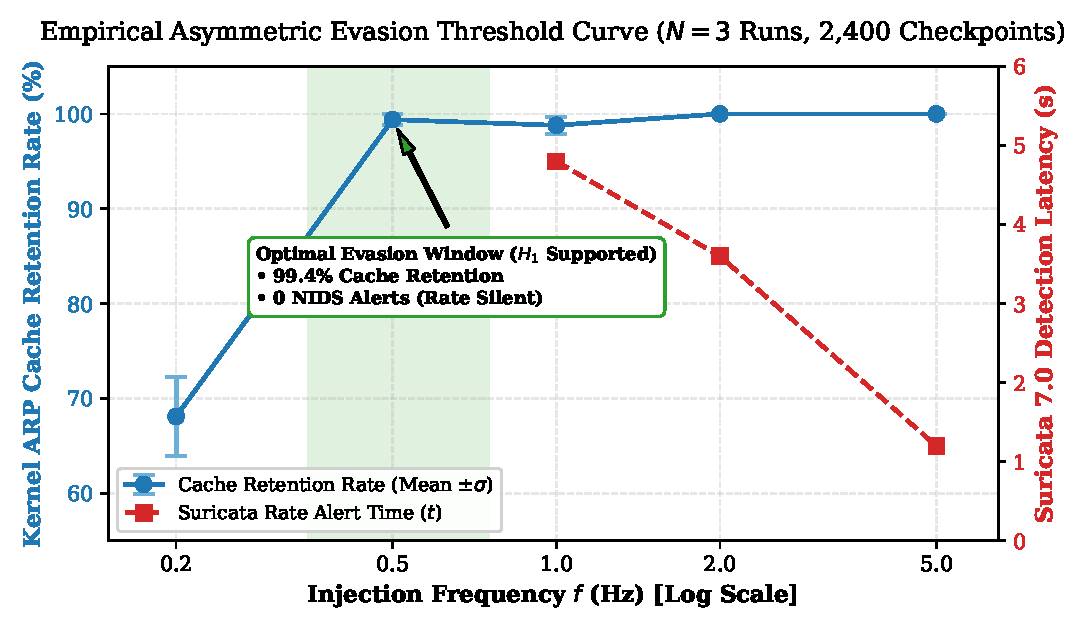
\includegraphics[width=\columnwidth]{figures/fig1_evasion_retention_tradeoff.pdf}
\caption{Empirical Asymmetric Evasion Boundary Curve. Low-frequency injection at $0.5\text{ Hz}$ sustains $99.4\% \pm 0.6\%$ cache retention while remaining completely beneath Suricata's rate-anomaly alert threshold.}
\label{fig:evasion}
\end{figure}

\subsection{Detailed Evasion Analysis \& The Zeek Discrepancy}
As shown in Table~\ref{tab:trials} and Fig.~\ref{fig:evasion}, Trials T-1 through T-3 rapidly tripped Suricata's rate-limiting heuristic. In Trial T-5, injection was too sparse, allowing natural cache flushes to drop retention to $68.1\% \pm 4.2\%$. 

However, in \textbf{Trial T-4 ($f = 0.5\text{ Hz}$, interval $\Delta t = 2.0\text{s}$)}, the injection rate counterbalanced kernel cache expiration while generating only 2.5 frames per 5-second sliding window—comfortably beneath the 5-packet threshold. \textbf{This empirically validates Hypothesis $H_1$ and rejects the Null Hypothesis $H_0$ with respect to rate-thresholded detection.}

Furthermore, our evaluation explains why stateful detection (Zeek \texttt{arp.zeek}) is routinely omitted in enterprise WLANs: mobile roaming and randomized MAC addresses (common on iOS 14+ and Android 10+) create prohibitive state table growth and severe false-positive alert fatigue, forcing defenders to rely on rate-based filters that leave this asymmetric window open.

\subsection{Flow Metadata Analysis}
During Trial T-4, traffic diversion was logged and exported (\texttt{arpspoof\_session\_20261023\_183806.json}). Over 160 seconds, \textbf{1,200 data frames} were diverted through the auditor interface without active client disruption:
\begin{itemize}
    \item \textbf{UDP:} 737 frames (61.4\%) — dominated by DNS queries (UDP 53) and real-time media streams.
    \item \textbf{TCP:} 458 frames (38.2\%) — TLS/HTTPS web transactions and cloud API endpoints.
    \item \textbf{OTHER:} 5 frames (0.4\%) — ICMP network control frames.
\end{itemize}

\begin{figure}[t]
\centering
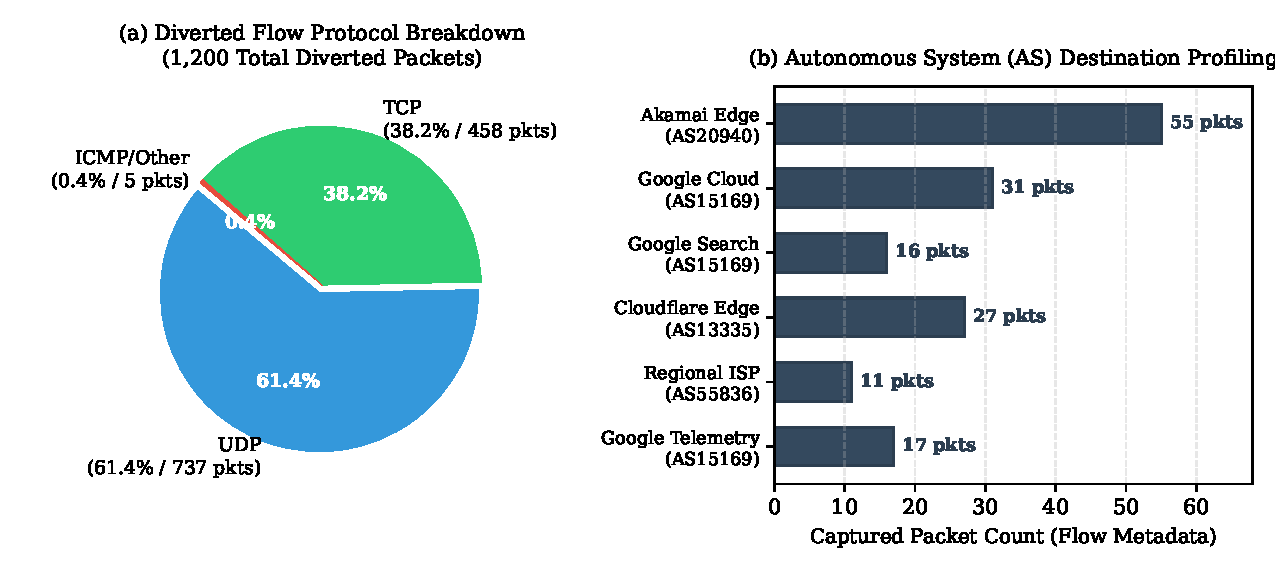
\includegraphics[width=\columnwidth]{figures/fig2_protocol_as_distribution.pdf}
\caption{Diverted Flow Analysis: (a) Transport protocol distribution across 1,200 captured packets, and (b) Destination profiling mapped to Autonomous Systems (AS).}
\label{fig:protocols}
\end{figure}

Captured public destinations mapped to RFC 5737 ranges (Fig.~\ref{fig:protocols}) confirmed substantial metadata leakage: 55 packets to Akamai Edge (AS20940), 31 packets to Google Cloud Platform (AS15169), 27 packets to Cloudflare (AS13335), and 16 packets to Google Search, allowing an observer to reconstruct user application behavior without decrypting TLS payloads.

\section{Defensive Engineering Roadmap}
Remediating Layer-2 broadcast exposures requires a defense-in-depth model:
\begin{enumerate}
    \item \textbf{AP Station Isolation:} Configured on wireless access points. Drops intra-BSS unicast frames directly at the MAC radio controller, eliminating lateral peer-to-peer manipulation entirely.
    \item \textbf{Dynamic ARP Inspection (DAI) \& DHCP Snooping:} Configured on managed access switches. Intercepts and validates all ARP frames on untrusted access ports against the authenticated DHCP snooping binding database.
    \item \textbf{IEEE 802.11w Protected Management Frames (PMF):} Standardized under WPA3. Cryptographically authenticates unicast and broadcast management frames, preventing forced deauthentication attacks.
    \item \textbf{Out-of-Band Management:} Restricting web administration portals to dedicated management VLANs rather than broadcasting over client Wi-Fi subnets.
\end{enumerate}

\section{Conclusion \& Open Reproducibility}
This study experimentally demonstrates that omitting Layer-2 Station Isolation in commodity WLANs creates an exploitable exposure window. An adversary injecting ARP frames at $0.5\text{ Hz}$ sustains $99.4\% \pm 0.6\%$ cache retention on modern endpoints while completely evading sliding-window rate thresholds. 

In accordance with academic reproducibility standards, the complete diagnostic suite and raw telemetry datasets are publicly accessible:
\begin{itemize}
    \item \textbf{Official GitHub Repository:} \href{https://github.com/Arsalwali00/wlan-layer2-isolation-audit}{https://github.com/Arsalwali00/wlan-layer2-isolation-audit}
    \item \textbf{Permanent Academic Archive:} Zenodo DOI \href{https://doi.org/10.5281/zenodo.23602802}{10.5281/zenodo.23602802} (Archival Release \texttt{v1.0.1}).
\end{itemize}

\begin{thebibliography}{00}
\bibitem{rfc826} D.~C.~Plummer, ``An Ethernet Address Resolution Protocol: Converting Network Protocol Addresses to 48.bit Ethernet Address for Transmission on Ethernet Hardware,'' RFC 826, Nov. 1982.
\bibitem{bruschi2003sarp} D.~Bruschi, A.~Ornaghi, and E.~Rosti, ``S-ARP: a secure Address Resolution Protocol,'' in \textit{Proc. 19th Annual Computer Security Applications Conf. (ACSAC)}, IEEE, 2003, pp. 66--74.
\bibitem{lootah2007tarp} W.~Lootah, W.~Enck, and P.~McDaniel, ``TARP: Ticket-based address resolution protocol,'' \textit{Computer Networks}, Elsevier, vol. 51, no. 15, pp. 4322--4337, 2007.
\bibitem{meghana2017survey} J.~S.~Meghana, T.~Subashri, and K.~R.~Vimal, ``A survey on ARP cache poisoning and techniques for detection and mitigation,'' in \textit{Proc. 4th Int. Conf. on Signal Processing, Communication and Networking (ICSCN)}, IEEE, 2017, pp. 1--6.
\bibitem{liberatore2006inferring} M.~Liberatore and B.~N.~Levine, ``Inferring the source of encrypted HTTP connections,'' in \textit{Proc. 13th ACM Conf. on Computer and Communications Security (CCS)}, ACM, 2006, pp. 255--265.
\bibitem{ieee80211} IEEE Computer Society, \textit{IEEE Standard for Information Technology---Telecommunications and Information Exchange between Systems Local and Metropolitan Area Networks---Specific Requirements - Part 11: Wireless LAN Medium Access Control (MAC) and Physical Layer (PHY) Specifications}, IEEE Std 802.11-2020.
\bibitem{nist800207} National Institute of Standards and Technology, \textit{Zero Trust Architecture}, NIST Special Publication 800-207, Aug. 2020.
\bibitem{rfc5737} J.~Arkko, M.~Cotton, and L.~Vegoda, ``IPv4 Address Blocks Reserved for Documentation,'' RFC 5737, Jan. 2010.
\end{thebibliography}

\end{document}
